

% Author: Dun-Ming Huang
% Email: dunmingbrandonhuang@berkeley.edu
% CSM16A Fall 2022
\qns{YEARS OF CIRCUITING yet NO REAL WORLD USE FOUND FOR censoring your roommate}

\textbf{Learning Goal}: Learn to use appropriate op-amp architectures, correct methods to piece designed elements and blackboxes to form circuits. \\
\meta{
    \begin{bindenum}
        \item \textbf{Remind students to buffer} when parts of circuits are to collide and interfere with each other.
        \item Can \textbf{adapt a process of elimination to choose for the  op-amp architecture} from the toolkit.
        \item \textbf{Have the behaviour of comparator} memorized and ready so it is \textbf{easier to revise and build circuits by making analogies to it}.
    \end{bindenum}
}

Obviously, circuitry comes with its benefits, as it is the great foundation of all things electrical engineering. Using circuits, humanity has accomplished a lot of great things. Circuits themselves become more complicated, and the unit "Operational Amplifier" has invented from this evolutionary history of circuit elements. It makes us wonder what great things can be born from these technological advancements!

For me, I want to censor my roommate Winston when I need to work quietly using circuit elements. Here's how it works:

\begin{enumerate}
    \item{
        First of all, I have the following blackboxes and circuit units from Cory Hall:
        \begin{center}
            % Author: Dun-Ming Huang
% Email: dunmingbrandonhuang@berkeley.edu
% CSM16A Fall 2022
% Code for operational amplifier and comparator comes from q_comparators.tex of CSM16A

\begin{circuitikz}
    \draw (0,0) node[op amp,yscale=-1] (opamp) { }
      (-2.5, 0.5) to [short, i=$i_{+}$, o-] (opamp.+) 
      (-2.5, -0.5) to [short, i=$i_{-}$, o-] (opamp.-) 
      (opamp.out) node[right ] {$V_{out}$} 
      ;
    \node[draw=none,text=black] at (-2.8, 0.5) {$V_{+}$};
    \node[draw=none,text=black] at (-2.8, -0.5) {$V_{-}$};
    \draw (-0.2, -0.2) to [short] (0, -0.2) to [short] (0, 0.2) to [short] (0.2, 0.2);
    \draw (0, 0.5) to [short, -o] (0, 1.0);
    \node[draw=none,text=black] at (0, 1.5) {$V_{DD}$};
    \draw (0, -0.5) to [short, -o] (0, -1.0);
    \node[draw=none,text=black] at (0, -1.5) {$V_{SS}$};
    
    \draw[draw=black] (-11, -0.5) rectangle (-8, 0.5);
    \node[] at (-9.5, 0) {Sound Sensor};
    
    \draw (-8, 0) to [short] (-7.5, 0);
    
    \draw[draw=black] (-7.5, -0.5) rectangle (-3.5, 0.5);
    \node[] at (-5.5, 0) {Sound-Volt Converter};
    
    \draw (-3.5, 0) to [short, -o] (-3, 0);
    
    \draw
        (3, -1) to [V, l^=$3V$, invert] (3, 1)
        (4.5, -1) to [V, l^=$5V$, invert] (4.5, 1);
\end{circuitikz}
        \end{center}
        I will use a comparator because it is strong in providing binary outputs based on an input.
        \begin{center}
            %Code Referenced from q_review_opamps.tex

% Author: Dun-Ming Huang
% Email: dunmingbrandonhuang@berkeley.edu
% CSM16A Fall 2022

\begin{center}
    Comparator Behaviour be like: \\
    \begin{tikzpicture}
        \begin{axis}[
            axis lines = middle,
            xlabel = {$U_+$},
            ylabel = {$V_{out}$},
            legend pos=outer north east,
            legend cell align=left
        ]
            \addplot [color=red, domain=0:5] {
               5
            };
            \addlegendentry{$V_{DD}$}
            \addplot [color=blue, domain=-5:0] {
               0
            };
            \addlegendentry{$V_{SS}$}
            \addplot +[mark=none, color=yellow] coordinates {(0, -6) (0, 6)};
            \addlegendentry{$U_- = 0V$}
        \end{axis}
    \end{tikzpicture}
\end{center}
        \end{center}
        I also know that my roommate's voice would always be characterized as any voltage below $3V$. Using this knowledge, and assuming you have any amount of wires you'd like, draw out a circuit involving all elements above that outputs $5V$ for any voice input $V_{in}$ that is not possibly my roommate's, and $0V$ otherwise.
        
    }
    \ans{
        For any voltage above $3V$, then, it must not be the roommate's voice. Therefore, the behaviour of this circuit can be portrayed as:
        \[
            V_{out} = 
            \begin{cases}
                5V, &V_{in} > 3V \\
                0V, &V_{in} < 3V
            \end{cases}
        \]
        The behaviour of a comparator, meanwhile, may be portrayed as:
        \[
            V_{out} = 
            \begin{cases}
                V_{DD}, &V_+ > V_- \\
                V_{SS}, &V_+ < V_-
            \end{cases}
        \]
        Let us make analogy between the behaviours listed above, keep in mind that $V_{in}$ is the voltage from Sound-Volt Converter, and we may construct the following circuit:
        \begin{center}
            % Author: Dun-Ming Huang
% Email: dunmingbrandonhuang@berkeley.edu
% CSM16A Fall 2022
% Code for operational amplifier and comparator comes from q_comparators.tex of CSM16A

\begin{circuitikz}
    \draw (0,0) node[op amp,yscale=-1] (opamp) { }
      (opamp.out) node[right ] {$V_{out}$} 
      ;
	\draw (-0.2, -0.2) to [short] (0, -0.2) to [short] (0, 0.2) to [short] (0.2, 0.2);
    \draw
        (0, 0.5)
            to [short] (0, 1.0)
            to [V, l^=$5V$] (2, 1) node[ground]{}
        ;
    \node[draw=none,text=black] at (0, 2) {$V_{DD}$};
    \draw (0, -0.5) to [short] (0, -1.0) node[ground]{};
    \node[draw=none,text=black] at (0, -2) {$V_{SS}$};
    
    \draw[draw=black] (-11, 0) rectangle (-8, 1);
    \node[] at (-9.5, 0.5) {Sound Sensor};
    
    \draw (-8, 0.5) to [short] (-7.5, 0.5);
    
    \draw[draw=black] (-7.5, 0) rectangle (-3.5, 1);
    \node[] at (-5.5, 0.5) {Sound-Volt Converter};
    
    \draw
        (-3.5, 0.5)
            to [short] (opamp.+)
        (-3.5, -0.5) node[ground]{}
            to [V, invert, l_=$3V$] (opamp.-)
        ;
\end{circuitikz}
        \end{center}
        In such a circuit:
        \[
            V_{out} = 
            \begin{cases}
                V_{DD} = 5V, &V_+ = V_{in} > V_- = 3V \\
                V_{SS} = 0V, &V_+ = V_{in} < V_- = 3V
            \end{cases}
        \]
        
    }
    
    \item{
        My roommate decided to interfere and piece all my circuit elements into something below, which, as a 16A Content Mentor, I can't quite tell what's going on with:
        \begin{center}
            \begin{center}
    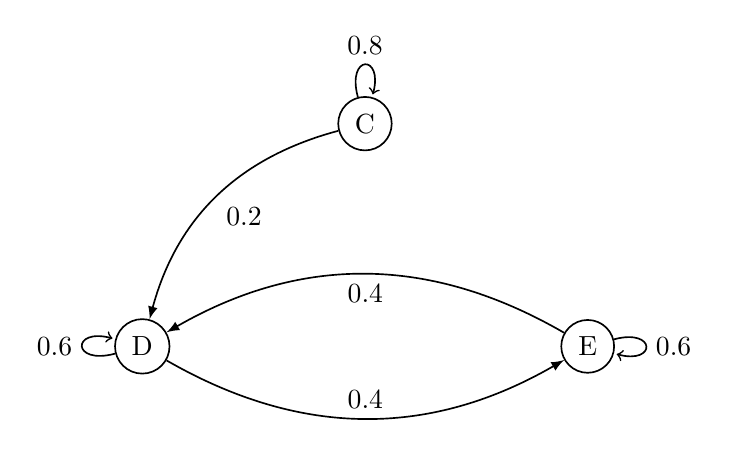
\begin{tikzpicture}[-latex, auto, node distance={4cm}, semithick, main/.style = {draw, circle}]
        \node[main] (C) {C};
        \node[main, below left of = C] (D) {D};
        \node[main, below right of = C] (E) {E};
        \path (C) edge[loop above] node{0.8} (C);
        \path (C) edge[bend right] node{0.2} (D);
        \path (D) edge[loop left] node{0.6} (D);
        \path (D) edge[bend right] node{0.4} (E);
        \path (E) edge[bend right] node{0.4} (D);
        \path (E) edge[loop right] node{0.6} (E);
    \end{tikzpicture}
\end{center}


        \end{center}
        Explain what the above circuit is doing.
    
    }
    \ans{
        Let us briefly summarize this circuit according to the comparator behavior:
        \[
            V_{out} = 
            \begin{cases}
                V_{DD}, &V_+ > V_- \\
                V_{SS}, &V_+ < V_-
            \end{cases}
        \]
        \[
            V_{out} = 
            \begin{cases}
                4V, &\frac{1}{4} V_{in} > 0 \\
                2V, &\frac{1}{4} V_{in} < 0
            \end{cases}
        \]
        
    }
    
    \item{
        Unfortunately, this filter happened to also filter out everyone who has a similar voice to my roommate's. However, using perfect pitch, I discovered that my roommate's voice has a specific frequency to it. \\
        I turned to a different design, but need to first process the output of sound-to-volt converter. \\
        For an input voltage of $V(t)$, I would like to transform it into $V'(t) = -0.5V(t) + 2$. \\
        Draw a circuit involving an input node, output node, and an op-amp architecture that enables it. As an additional constraint, you are also only given an op-amp, infinite wires, and can use some of the following basic circuit components:
        \begin{center}
            % Author: Dun-Ming Huang
% Email: dunmingbrandonhuang@berkeley.edu
% CSM16A Fall 2022

\begin{circuitikz}
    \draw
        (-3, 0) to [R, l^=$1k\Omega$] (-3, 1)
        (-1.5, 0) to [R, l^=$2k\Omega$] (-1.5, 1)
        (0, 0) to [R, l^=$2k\Omega$] (0, 1)
        (1.5, 0) to [R, l^=$3k\Omega$] (1.5, 1)
        (3, 0) to [R, l^=$3k\Omega$] (3, 1)
        (5, 0) to [V, l_=$1V$, invert] (5, 1)
        ;
\end{circuitikz}

        \end{center}
    
    }
    \ans{
        In this case, since the voltage is being converted into some opposite sign, I can use an inverting amplifier:
        \begin{center}
            %Code Referenced from q_review_opamps.tex

\begin{circuitikz}
	\draw
	(0,0) node[op amp] (AMP) {}
	(AMP.-) to[short] ++(0,1) coordinate (topLeft)
		to[R,l=$R_f$] (topLeft -| AMP.out)
		to[short] (AMP.out)
		to[short,-o] ++(1,0)
		to[open,o-o,v^=$v_\text{out}$] ++(0,-2)
		node[ground] () {}
	(AMP.-) to[R,l_=$R_s$] ++(-2,0)
		to[sV,v_=$v_\text{in}$] ++(0,-2)
		node[ground] () {}
	(AMP.+) to[V, v_=$V_{ref}$] ++(0,-1.5)
		node[ground] () {};
\end{circuitikz}
\[V_{out} = -\frac{R_f}{R_s} V_{in} + \bigg( \frac{R_f}{R_s} + 1\bigg) V_{ref}\]

        \end{center}
        Notice that such an amplifier is incapable of shrinking voltage. Therefore, my circuit should feed the voltage signal to an inverting amplifier that, after inverting its sign and halving it, adds $2V$ to it. \\
        Since the $1V$ voltage source is out only available voltage source, and we do need a $V_{ref}$ to add the $2V$, it would have to be $V_{ref}$. \\
        Now, to build such an inverting amplifier, we would most definitely need:
        \[\frac{R_f}{R_s} = \frac{1}{2}\]
        But, by doing so, the added voltage after halving and inverting becomes
        \[\bigg( \frac{R_f}{R_s} + 1\bigg) V_{ref} = \frac{3}{2} V\]
        Which is not $2V$. \\
        Consider the alternative then, where we, to secure
        \[\bigg( \frac{R_f}{R_s} + 1\bigg) V_{ref} = 2V\]
        enforce that
        \[\frac{R_f}{R_s} = \frac{1}{1}\]
        And let the circuit follow the procedure of:
        \begin{bindenum}
            \item Halving the voltage input $V(t)$.
            \item Feed the halved signal to the inverting op-amp, inverting its sign and then add $2$ to it, resulting in $-0.5V(t) + 2V$.
        \end{bindenum}
        If so, we would just need a voltage divider to perform the first step, which would take 2 resistors of the same resistance. Since we are using a voltage divider, we would like to introduce a buffer between it and the op-amp architecture as well to avoid external influence. \\
        Therefore, the entire circuit would look like this:
        \begin{center}
            % Author: Dun-Ming Huang
% Email: dunmingbrandonhuang@berkeley.edu
% CSM16A Fall 2022
\includegraphics[scale=0.8]{../../topics/resistors/q_resist_design_figs//four_buttons.png}
\hspace{5mm}
\begin{circuitikz}[american, scale=0.8]
    \draw
        (-2, -0.3) node[ground]{}
        to [short] (-2, 4)
        (-2, 1)
        to [V, l_=$5V$, invert] (1, 1)
        to [short, -o] (1.05, 1)
        (-2, 2)
        to [V, invert] (1, 2)
        to [short, -o] (1.25, 2)
        (-2, 3)
        to [V, invert] (1, 3)
        to [short, -o] (1.05, 3)
        (-2, 4)
        to [V, invert] (1, 4)
        to [short] (4, 4)
        to [short, -o] (4, 3.5)
        (4, 1)
        to [rmeter, t=Dig, i=$i_{Dig}$] (4, -0.3) node[ground]{}
        (3.2, 3)
        to [short, o-] (3.5, 3)
        to [short] (3.5, 1)
        to [short, -o] (3.2, 1)
        (3, 2) to [short, o-] (3.5, 2)
        (3.5, 1.5)
        to [short] (4, 1.5)
        to [short] (4, 1)
        (4, 1.5) to [short, -o] (4, 1.6)
        (1.05, 3) to [R, l^=$R_Y$, i=$i_Y$] (3.2, 3)
        (1.25, 2) to [R, l^=$R_A$, i=$i_A$] (3, 2)
        (1.05, 1) to [R, l^=$R_B$, i=$i_B$] (3.2, 1)
        (4, 3.5) to [R, l^=$R_X$, i=$i_X$] (4, 1.6);
\end{circuitikz}
        \end{center}
    }
    
    \item{
        After the transformation from part (c), I would like to perform another transformation that transforms $V'(t)$ into $V''(t) = -V(t) + 1$. \\
        Suggest and draw a circuit involving an input node, output node, and an op-amp architecture that enables it. As an additional constraint, you are also only given an op-amp, infinite wires, and can use some of the following basic circuit components:
        \begin{center}
            % Author: Dun-Ming Huang
% Email: dunmingbrandonhuang@berkeley.edu
% CSM16A Fall 2022

\begin{circuitikz}
    \draw
        (1.5, 0) to [R, l^=$1k\Omega$] (1.5, 1)
        (3, 0) to [R, l^=$3k\Omega$] (3, 1)
        (7, 0) to [R, l^=\text{Any value you like}] (7, 1)
        (8, 0) to [V, l_=$3V$, invert] (8, 1)
        ;
\end{circuitikz}

        \end{center}
        
    }
    \ans{
        We are attempting to transform $-0.5 V(t) + 2$ into $-1 V(t) + 1$. \\
        This must be the work of a non-inverting amplifier! \\
        We can first double the entire $V'(t)$, which doubles the constant term into a $4V$, and then subtract $3V$ from the doubled signal. \\
        A non-inverting amplifier looks like this:
        \begin{center}
            %Code Referenced from q_review_opamps.tex

\begin{circuitikz}
	\draw
	(0,0) node[op amp] (AMP) {}
	(AMP.-) to[short] ++(0,1) coordinate (topLeft)
		to[R,l_=$R_{top}$] (topLeft -| AMP.out)
		to[short] (AMP.out)
	(AMP.out)
		to[short] ++(2,0)
		to[open,o-o,v^=$v_\text{out}$] ++(0,-2)
		node[ground] () {}
	(AMP.out)
	    to[short] ++(1,0)
	    to[R,l_=$R_{bottom}$] ++(0,-1.5)
	    to[V,v_=$V_{ref}$] ++(0,-1.5) node[ground]{}
	(AMP.+) to[sV,v_=$V_{in}$] ++(0,-1.5)
		node[ground] () {};
\end{circuitikz}
\[V_{out} = \bigg( \frac{R_{top}}{R_{bottom}} + 1\bigg) V_{in} + -\frac{R_{top}}{R_{bottom}} V_{ref}\]

        \end{center}
        Looking at this diagram, we first recognize that we must secure:
        \[\frac{R_{top}}{R_{bottom}} = 1\]
        to secure the signal's doubling. \\
        This works with the voltage source that we can use as $V_{ref}$, as this amplifier will then subtract $3V$ from the doubled signal. \\
        Therefore, the following architecture can work:
        \begin{center}
            %Code Referenced from q_review_opamps.tex

\begin{circuitikz}
	\draw
	(0,0) node[op amp] (AMP) {}
	(AMP.-) to[short] ++(0,1) coordinate (topLeft)
		to[R,l_=$R_1$] (topLeft -| AMP.out)
		to[short] (AMP.out)
	(AMP.out)
		to[short] ++(2,0)
		to[open,o-o,v^=$v_\text{out}$] ++(0,-2)
		node[ground] () {}
	(AMP.out)
	    to[short] ++(1,0)
	    to[R,l_=$R_1$] ++(0,-1.5)
	    to[V,v_=$3V$] ++(0,-1.5) node[ground]{}
	(AMP.+) to[short, -o] ++(0,-1.5)
		node[label=below:$V'(t)$] {};
\end{circuitikz}

        \end{center}
    }
\end{enumerate}
